\documentclass{article}

\usepackage{amsmath}
\usepackage{graphicx}
\usepackage{siunitx}
\usepackage{algorithm}
\usepackage[noend]{algpseudocode}
\usepackage[citestyle=ieee,sorting=none,bibencoding=utf8,backend=biber]{biblatex}
\usepackage{caption}
\usepackage[utf8]{inputenc}
\usepackage{hyperref}

\graphicspath{{figures/}}
\bibliography{bibliography}
\makeatletter
\def\BState{\State\hskip-\ALG@thistlm}
\makeatother

\author{J.R. Powers-Luhn}
\title{CS528 Project 2: PCA and K Means}
\date{October 22nd, 2018}

\begin{document}
	\maketitle
	
	\section{Objective}
	The goal of this project was to explore unsupervised clustering and means of evaluating the 
	clusters generated by the K-Means algorithm. The ability of Principal Component Analysis to 
	improve the performance of this algorithm was also explored.
	
	\section{Preprocessing the data}
	A dataset was obtained with several summary statistics for fifty seven U.S. universities, 
	mostly obtained from the Department of Education's Integrated Postsecondary Education Data System (IPEDS).
	
	The dataset was processed in several ways before numerical analysis. Two missing values for 
	Clemson University were obtained: the IPEDS ID number (from the IPEDS website) and the 2017 
	endowment balance\footnote{Source: \url{https://www.clemson.edu/giving/cufoundations/documents/allocations.pdf}}. 
	Some information (medical and agricultural school research funding) was absent for many schools 
	and was therefore removed from the data. None of the schools included in the dataset were 
	historically black colleges, so the ``HBC'' column had zero variance and was therefore removed. 
	Only some of the schools had Wall Street Journal rankings; this column was removed. Some columns 
	were determined to be categorical--these were ``one-hot'' encoded.
	
	For all processing in this project, the numerical attributes were mean-centered and scaled to 
	unit variance. This was accomplished using the scikit-learn \texttt{StandardScaler} class 
	\cite{scikit-learn}. Scaling is necessary due to the different units of the various measurements. 
	Without this correction the variance would be skewed by the units and mean value of the individual 
	measurements.
	
	\section{PCA}
	Principal component analysis (PCA) was applied to the data. PCA is a linear transformation of a 
	dataset into a new basis set. The principal components have the following properties:
	
	\begin{itemize}
		\item the components are orthogonal to each other, and
		\item the components are ordered by the amount of variance they exhibit.
	\end{itemize}
	
	This means that the dimensionality of the data can be reduced by transforming the data into the 
	new space (where the transformed values are referred to as ``scores'') and throwing away all but 
	\texttt{k} columns of the transformed data. 
	
	The transformation into the new space is performed by taking the singular value decomposition of 
	the original data as indicated in equation \ref{eq:svd}. 
	
	\begin{equation}
		\mathbf{U}, \mathbf{S}, \mathbf{V}^T = svd(\mathbf{X})
		\label{eq:svd}
	\end{equation}
	
	In equation \ref{eq:svd}, $\mathbf{US}$ is the transformed data, $\mathbf{S}$ are the singular 
	values, and $\mathbf{V}$ are the principal component loadings used to transform $\mathbf{X}$ into 
	the PC space. $\mathbf{S}$ is a diagonal matrix with the property that the diagonal values are 
	proportional to the amount of variance captured by the associated principal component. The number 
	of principal components to capture some fraction $f$ of the variance is shown in equation 
	\ref{eq:var_frac}.
	
	\begin{equation}
		\sum_{i=0}^k \vec{s^2} = f
		\label{eq:var_frac}
	\end{equation}
	
	For the university dataset, the data in its pre-processed form had sixty two numeric dimensions. 
	However, the vast majority of the variance was contained in the first few principal components, as 
	shown in figure \ref{fig:explained_variance}.
	
	\begin{figure}[h]
		\centering
		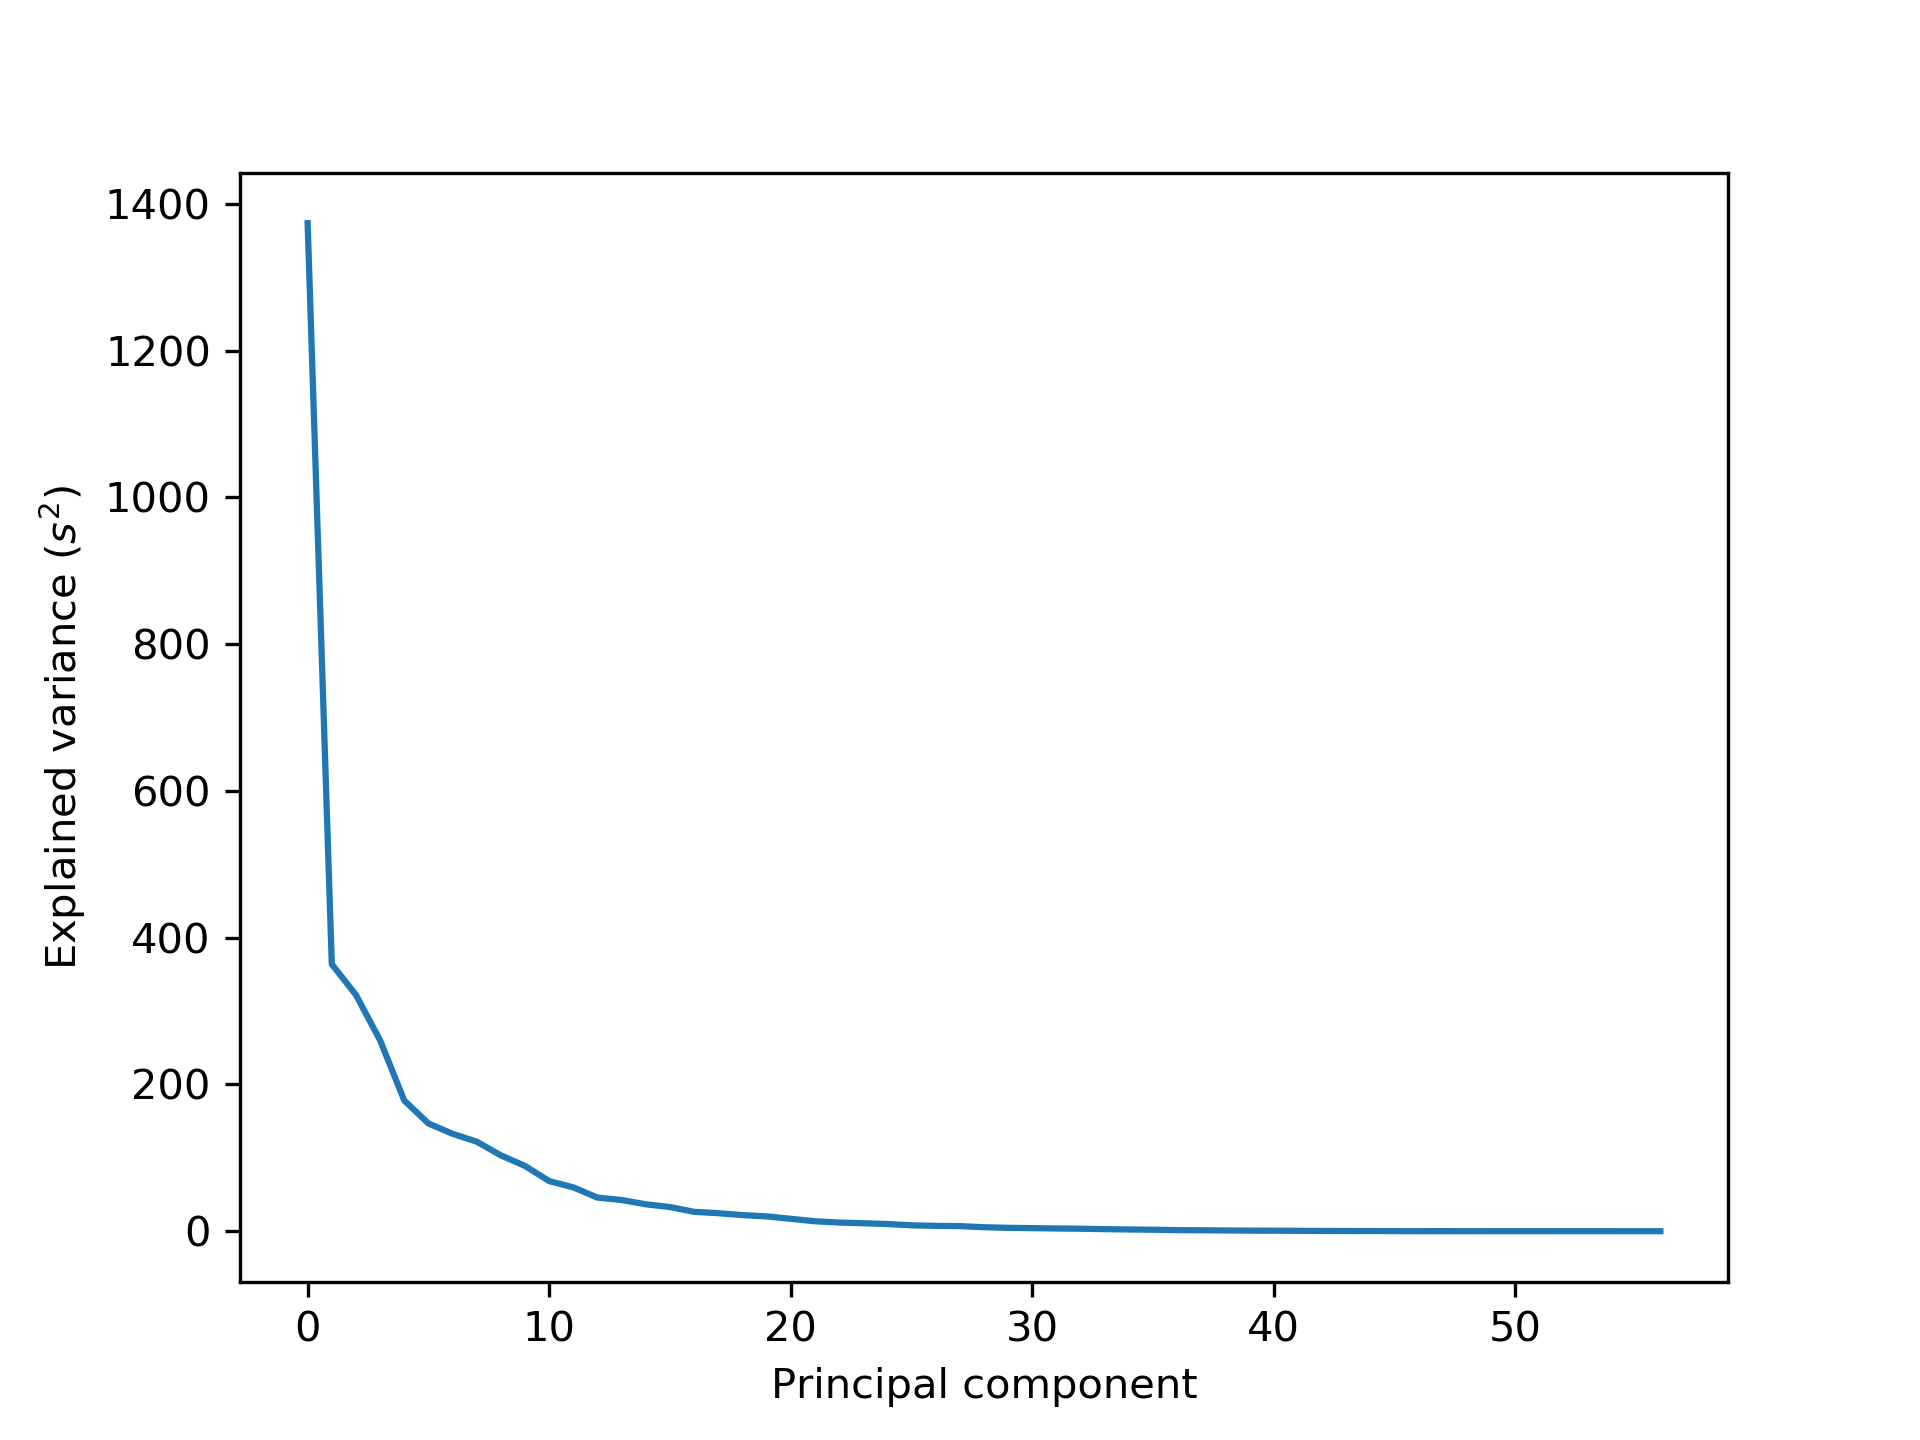
\includegraphics[width=0.8\textwidth]{explained_variance}
		\caption{Variance explained by each principal component (unscaled)}
		\label{fig:explained_variance}
	\end{figure}
	
	In order to simplify the dataset while retaining 95\% of the variance (and, therefore, the original 
	information), the cumulative sum of the singular values squared (normalized to the sum of the square 
	of all singular values) was calculated, and a threshold set at the first value that exceeded \num{0.95}.
	
	\begin{figure}[h]
		\centering
		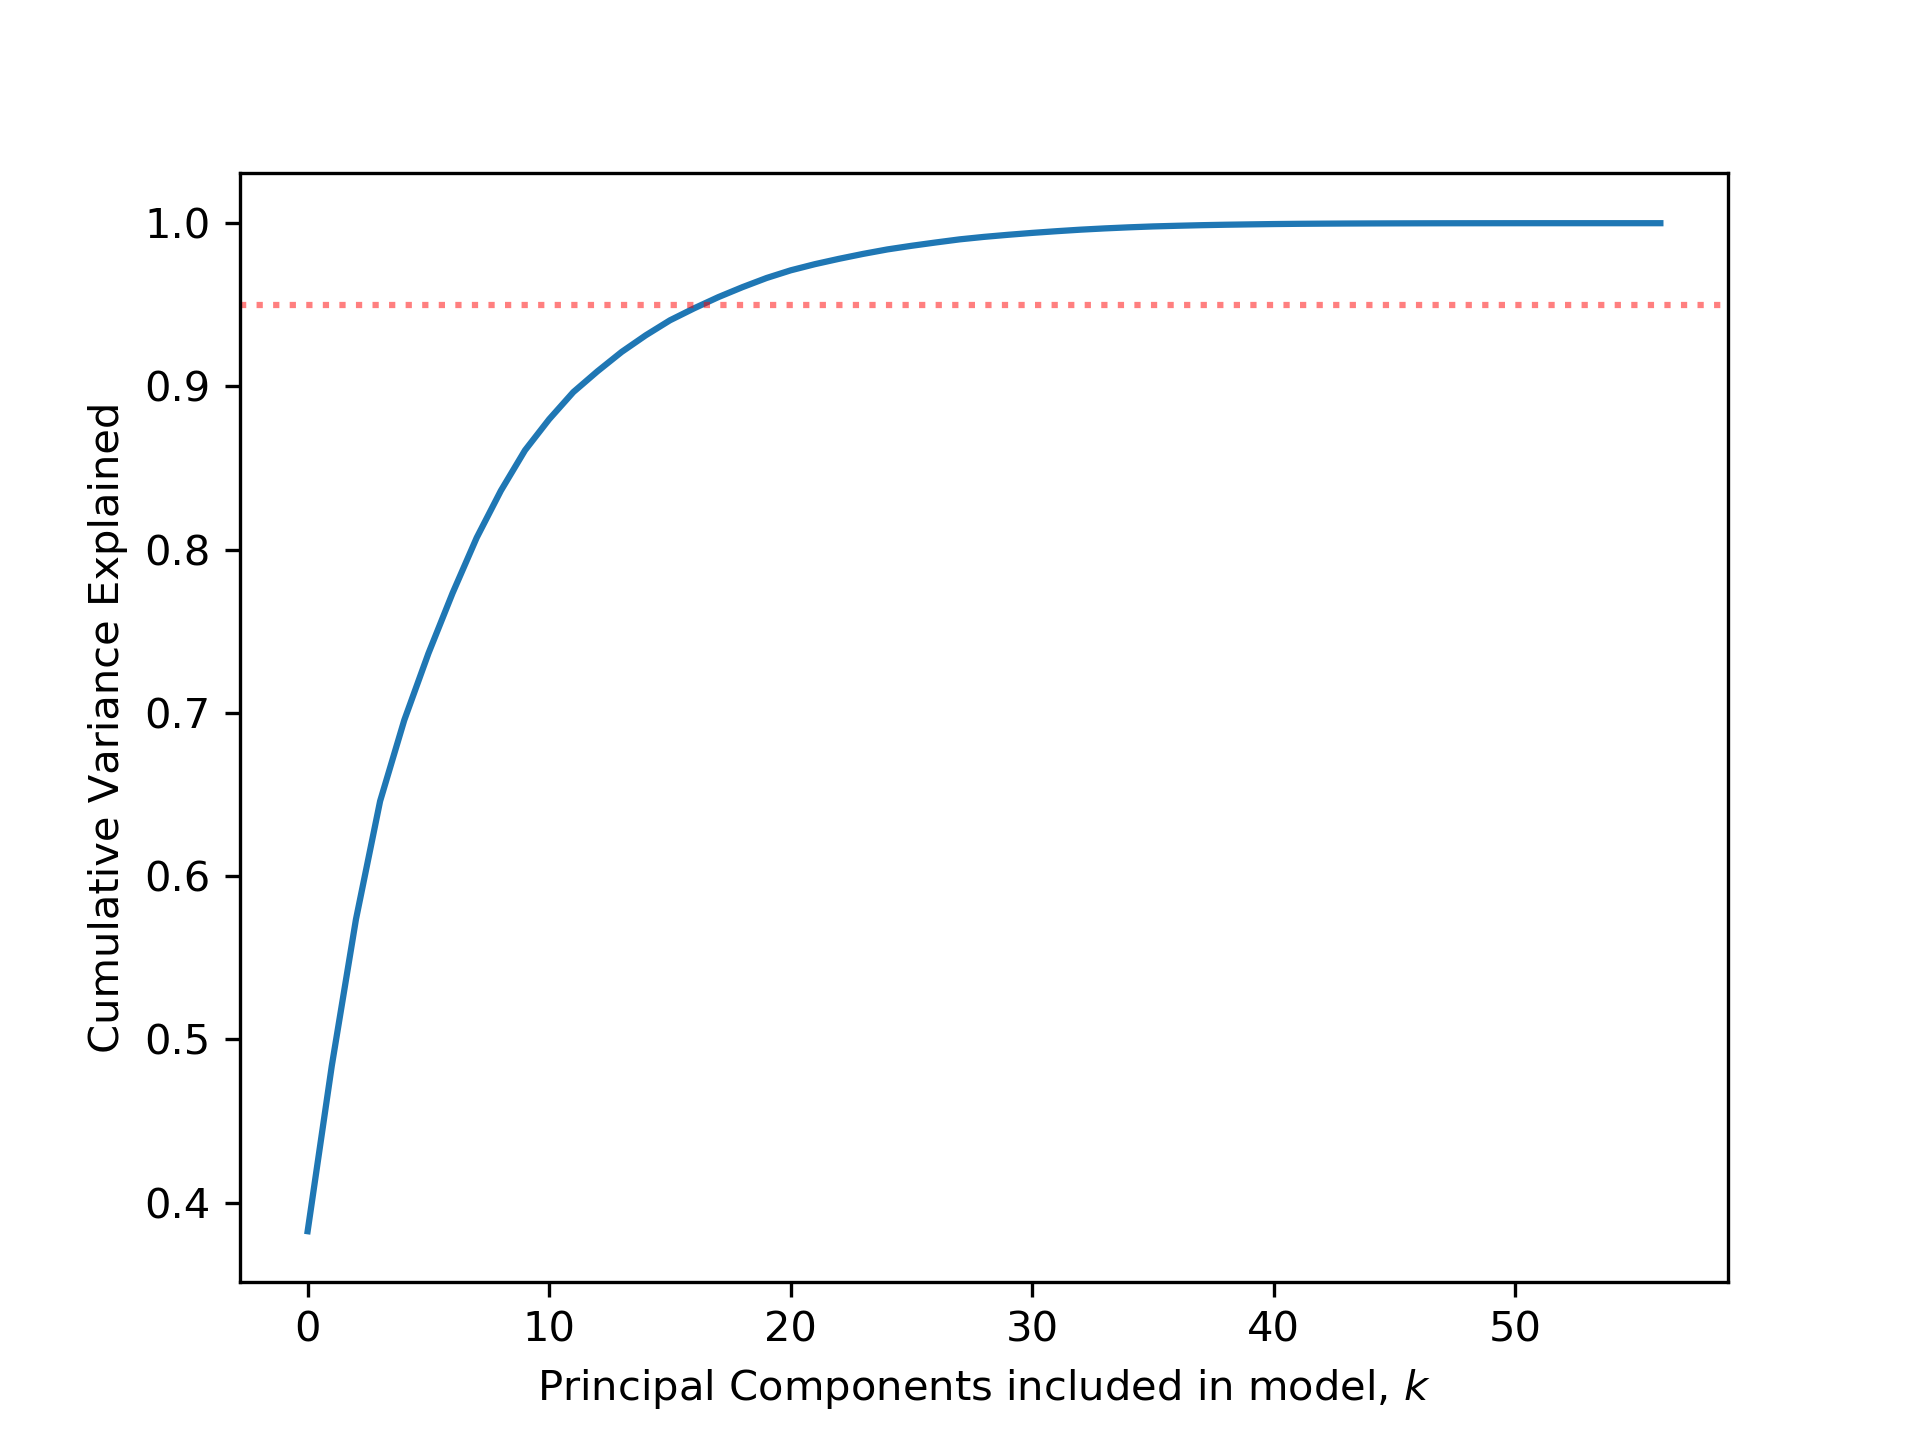
\includegraphics[width=0.8\textwidth]{cumulative_explained_variance}
		\caption{Cumulative variance explained by the first $k$ principal components}
		\label{fig:cumulative_explained_variance}
	\end{figure}
	
	As shown in figure \ref{fig:cumulative_explained_variance}, this corresponded to the first \num{17} 
	components. A scatter graph of the first two components plotted against each other is shown in 
	figure \ref{fig:pc1_vs_pc2}
	
	\begin{figure}[h]
		\centering
		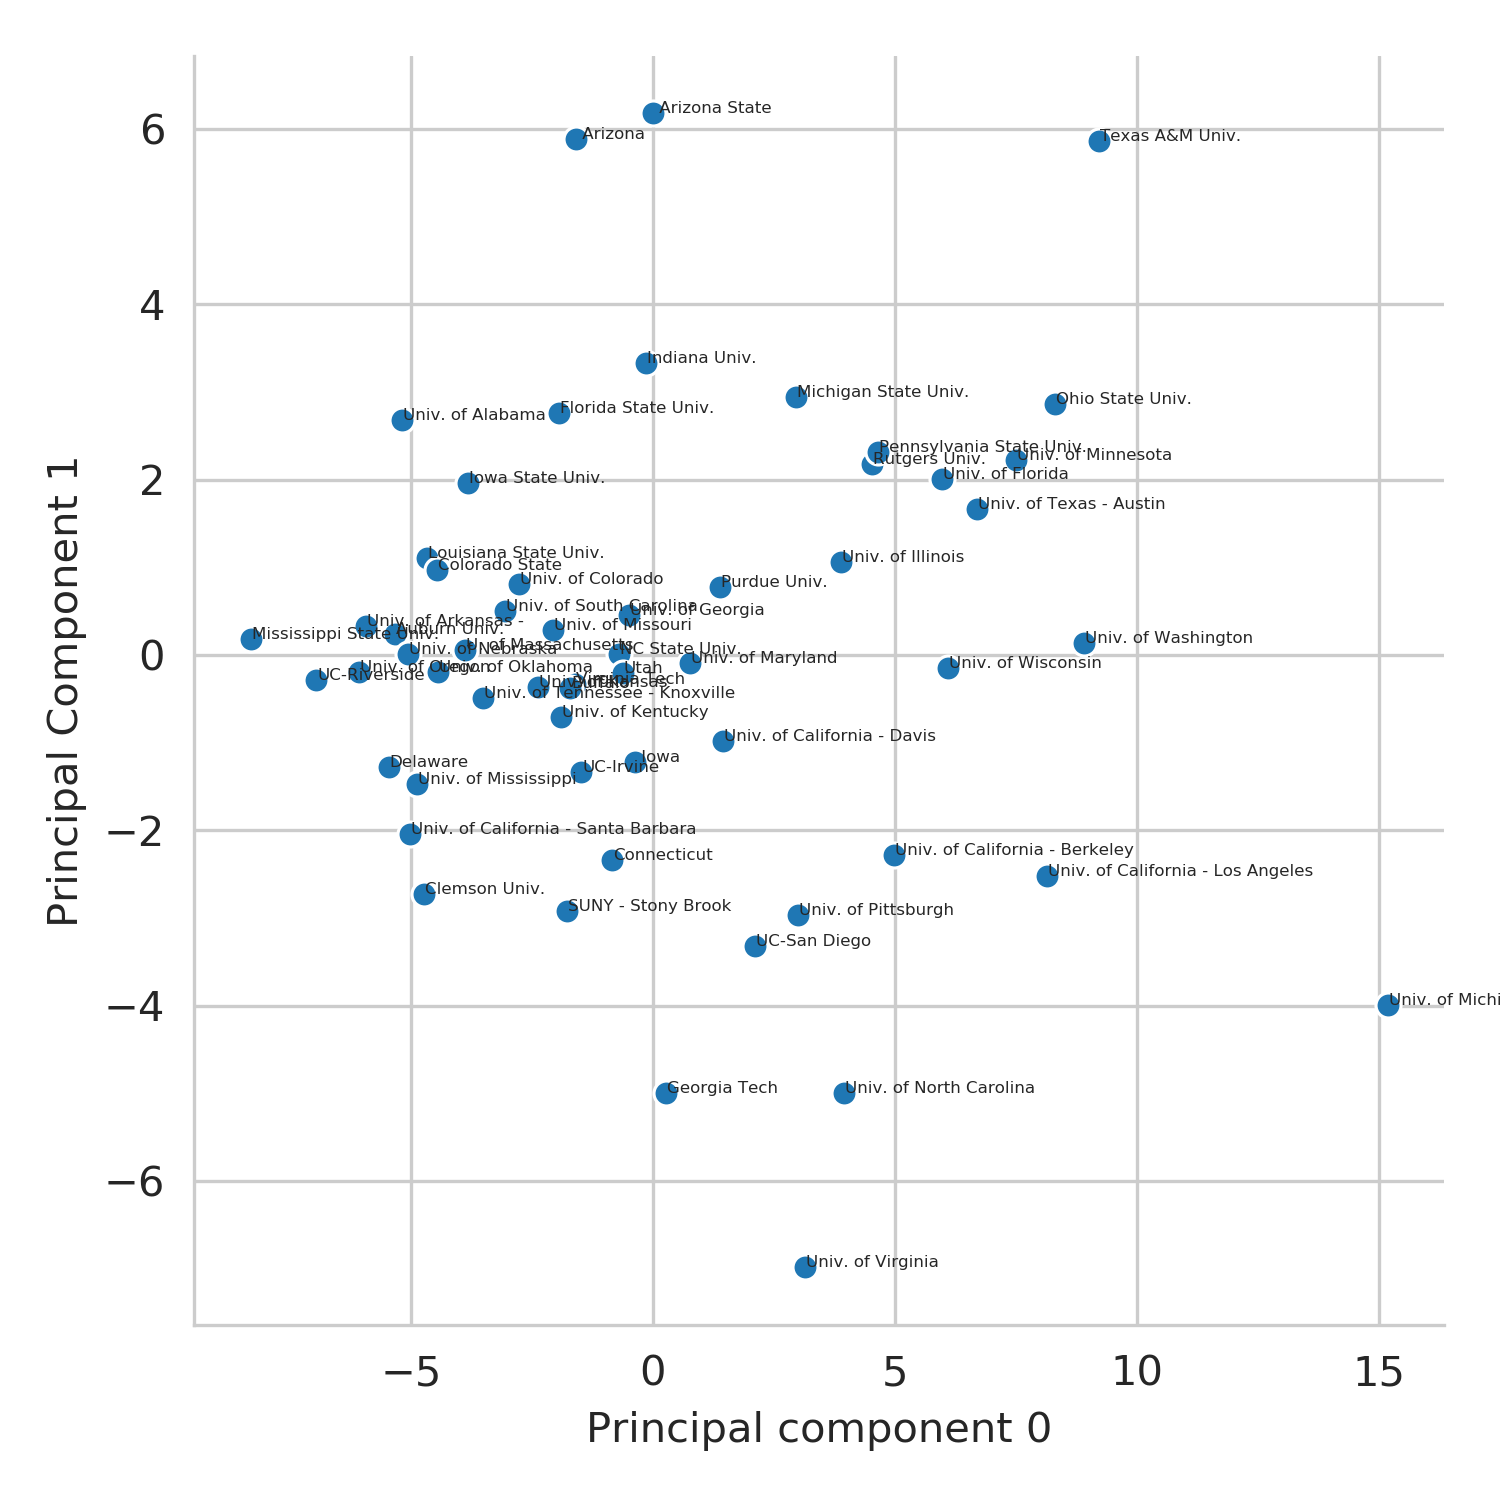
\includegraphics[width=0.8\textwidth]{pc1_v_pc2}
		\caption{The first two principal components plotted against each other. Since the PC's are 
				 orthogonal to each other, no linear relationship is apparent. Note the scales of the 
				 two different axes. Since PC1 captures more variance than PC2, this axis convers a 
				 larger range.}
		\label{fig:pc1_vs_pc2}
	\end{figure}
	
	\section{K-means}
	In order to determine whether the schools could be grouped into categories, the \texttt{k-means} 
	algorithm was employed.
	
	\begin{enumerate}
		\item Select $k$ initial vectors from the data as seeds, $s_i \in \{s_0, s_1, \mathellipsis, s_k\}$
		\item Calculate the distance from each $s_i$ to each vector
		\item Assign to each vector the label associated with the seed with the minimum distance to that vector
		\item Recalculate each $s_i = \frac{\sum_j x_j}{j}$ for all $x_j$ with label $i$
		\item Repeat 2-4 until the values of $s$ converge
	\end{enumerate}
	
	This algorithm was found to converge in less than ten iterations.
	
	This algorithm is not guaranteed to converge to the optimal solution since it is sensitive to the 
	selection of the initial seeds. Because of this, the algorithm was repeated several times in order to 
	improve the likelihood of optimal selection.
	
	\subsection{K-means++}
	While the \texttt{k-means} algorithm is guaranteed to converge, it is not guaranteed to converge to an 
	optimum value. Specifically, it is subject to the selection of the initial seed vectors. In order to 
	improve upon this, the \texttt{k-means++} algorithm was employed\cite{Arthur2007}. In this the first 
	seed $s_1$ is selected at random from the data. Subsequent seeds $s_2, \mathellipsis, s_k$ are selected 
	using a weighted probability proportional to the distance of each vector from the closest seed. In this 
	way the initial selection of seeds avoids selecting vectors that are too close to each other. The 
	\texttt{k-means++} algorithm therefore converges much more quickly than \texttt{k-means}, usually in 
	a single iteration.
		
	\subsection{Cluster selection}
	Ideally, data clusters should exhibit both tight grouping (minimal intra-cluster distance) and wide 
	separation (maximal inter-cluster distance). The ratio of these two values (the minimum inter-cluster 
	distance to the maximum intra-cluster distance) is referred to as the ``Dunn Index'' \cite{dunn1974}. 
	Because the \texttt{k-means} algorithm is not guaranteed to converge to the optimal solution, the 
	Dunn Index is subject to the random selection of the initial vector. Still, it provides a tool for 
	evaluating the ``true'' number of clusters in the data.
	
	The \texttt{k-means} algorithm was applied to the data with $k$ ranging from \numrange{2}{56}. In each 
	case the clusters were allowed to converge and the Dunn index was calculated. The results are shown 
	in figure \ref{fig:dunn_index_raw_data}.
	
	\begin{figure}[h]
		\centering
		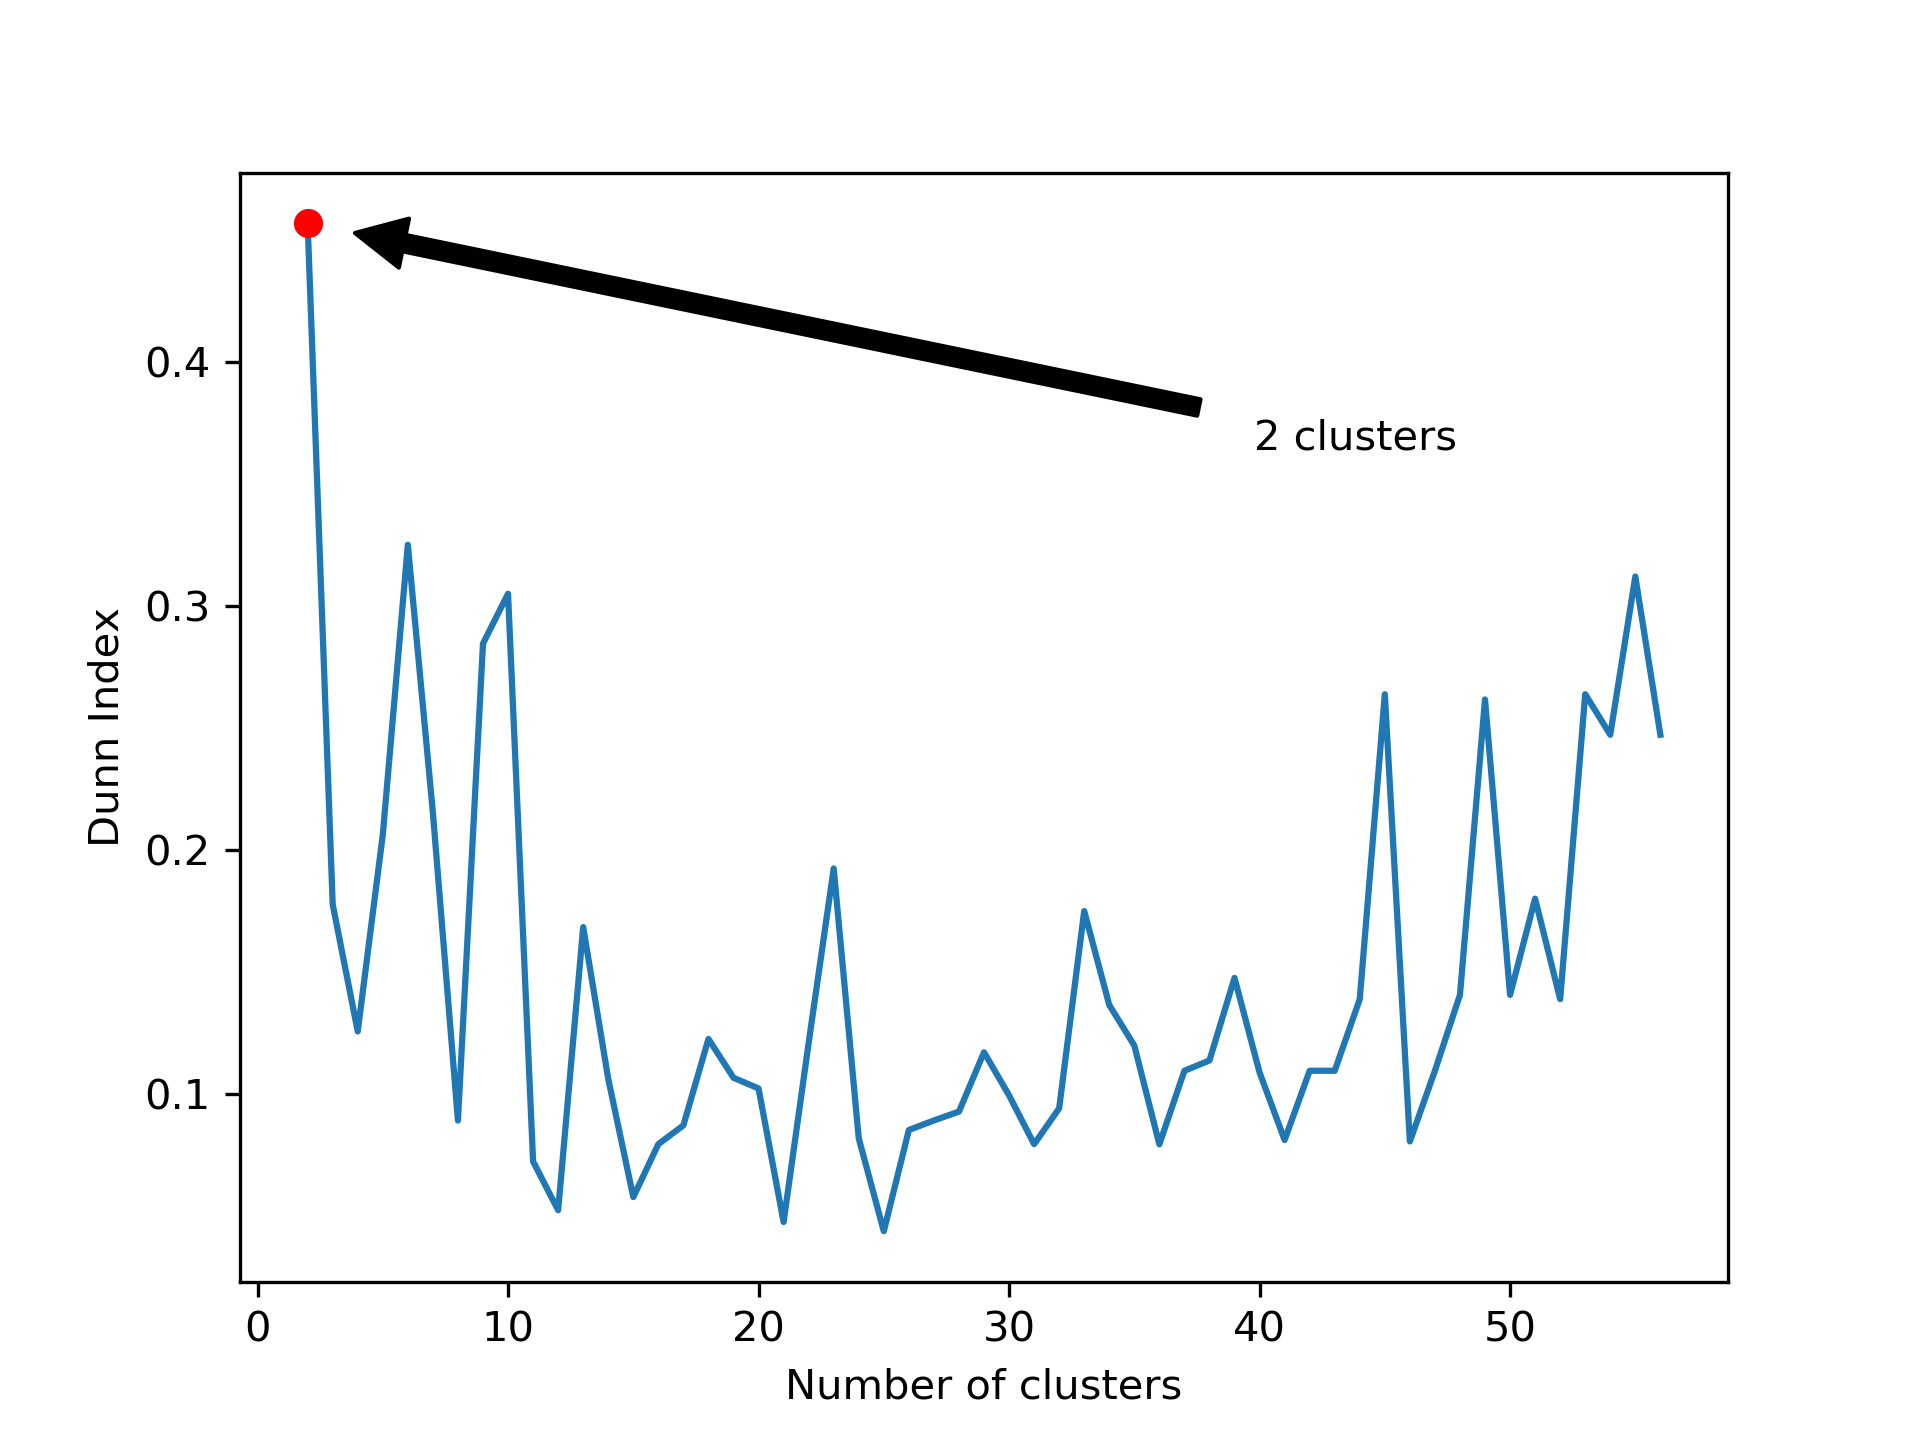
\includegraphics[width=0.8\textwidth]{dunn_index_raw_data}
		\caption{Dunn index for $k$ clusters. The value oscillates but has a clear maximum.}
		\label{fig:dunn_index_raw_data}
	\end{figure}
	
	Unfortunately, the Dunn index did not converge to a consistent maximum. Therefore an appropriate value 
	was chosen for the number of clusters that ``looked right''.
	
	
	
	\section{PCA plus K-Means}
	Lorem ipsum dolor simet \cite{Yeung2000}
	
	\section{Conclusions}
	Lorem ipsum dolor simet
		
	\printbibliography
\end{document}
